\chapter{能量守恒}

\section{什么是能量}

讲完对事物的一般性描述后,从这一章起,我们开始比较详细地研究物理学中各个方面的问题。为了说明理论物理学中可能用到的概念和推理的类型,我们现在来考查能量守恒定律,它是物理学:最基本的定律之一。

有一个事实,如果你愿意的话,也可以说一条\uwave{定律},支配着至今我们所知道的一切自然现象。没有发现这条定律有什么例外——就我们所知,它是完全正确的。这条定律称为\uwave{能量守恒定律}。它指出,在自然界所经历的种种变化之中,有一个称之为能量的物理量是不变的。那是一个最抽象的概念,因为它是一种数学原理;说的是在某种情况发生时,有一个数量是不变的。它并不是一种对机制或者具体事物的描写,而只是一件奇怪的事实。起先我们可以计算某种数值,当我们看完了大自然耍弄的技巧表演后,再计算一次数值,其结果是相同的。(有点类似于在红方格中的象,移动了几步后——具体步骤并不清楚——它仍然在某个红方格里。我们这条定律就是这种类型的定律。)由于这是一种抽象的概念,我们将用一个比喻来说明它的含义。

设想有一个孩子,或许就叫他“淘气的丹尼斯(Dennis)”,他有一堆积木,这些积木是绝对不会损坏的,也不能分成更小的东西。每一块都和其余的相同。让我们假定他共有28块积木。每天早上他的母亲把他连同28块积木一起留在一个房间里。到了晚上,母亲出于好奇心很仔细地点了积木的数目,于是发现了一条关于现象的规律——无论丹尼斯怎样玩积木,积木数目仍旧是28块!这种情况继续了好几天。直到有一天她发现,积木只有27块了,但是稍许调查一下就发现在地毯下面还有一块——为了确信积木的总数没有改变,她必须到处留神。然而,某一天积木的数目看来有些变化,只有26块了!仔细的调查表明:窗户已经打开,再朝窗外一看,就发现了另外的两块积木。又有几天,经过仔细的清点表明总共有30块积木!这使她相当惊愕,以后才了解到布鲁斯(Bruce)这个孩子曾带着他的积木来玩过,并留了几块在丹尼斯的房间里。自从丹尼斯的母亲拿走了多余的积木,把窗关上,并且不再让布鲁斯进来以后,一切都很正常,直到有一次,她清点时发现只有25块积木。然而,在房间里有一个玩具箱,母亲走过去打开这个箱子,但是孩子大声叫喊道:“不,别打开我的箱子,”不让她打开玩具箱。这时母亲十分好奇,也比较机灵,她想出了一种办法,她知道—块积木重3英两,有一次当她看到积木有28块时曾经称过箱子的重量为16英两,这一次她想核对一下,就重新称一下箱子的重量,然后减去16英两,再除以3,于是就发现了以下的式子:
\begin{equation}
    \label{Eq:I:4:1}
    \text{(所见到的积木数)}
    +
    \frac{\text{(箱重)}-\text{$16$ 英两}}{\text{$3$ 英两}}=
    \text{常数}.
\end{equation}
接着,又好像出现了某种新的偏差,但是仔细的研究又指出,浴缸里的脏水的高度发生了变化,孩子正在把积木扔到水里去,只是她看不见这些积木,因为水很混浊,不过在她的公式里再添上一项她就可以查明在水中有几块积木。由于水的高度原来是6英寸,每一块积木会使水升高$1/4$英寸,因而这个新的公式将是:
\begin{align}
    \label{Eq:I:4:2}
    \text{(所见到的积木数)}
    +
    \frac{\text{(箱重)}-\text{$16$ 英两}}{\text{$3$ 英两}}
    \frac{\text{(水的高度)- $6$英存}}{\text{$1/4$ 英寸}}+
    =
    \text{常数}.
\end{align}
在她这个复杂性逐渐增加的世界里,她发现了—系列的项来表示计算积木的方法,这些积木藏在不准她去看的那些地方。结果,她得出了\uwave{一个用于计算数量}的复杂公式,无论孩子怎样玩耍,这个量总是不变的。

这件事情和能量守恒有什么相似的地方呢?抽象地说,必须从这个图像中除去的最显著的一点就是,\uwave{根本没有积木}。在(\ref{Eq:I:4:1})及(\ref{Eq:I:4:2})中取走第一项,我们就会发现自己是在计算多少是有点抽象的东西。上述比较的相似之处在于以下几点。第一,当我们计算能量时,有时其中的一部分离开系统跑掉了,有时又有另一些能量进入这个系统。为了验证能量的守恒,必须注意我们没有把能量引入系统中或从系统中取走能量。第二,能量有许多\uwave{不同的形式},对每一种形式都有一个公式。这些不同形式的能量是:重力势能、动能、热能、弹性能、电能、化学能、辐射能、核能、质能。假如我们把表示这些能量的公式全都加在一起,那么,除非有能量逸出或有其他能量加入,否则其总和是不会改变的。

重要的是要认识到:在今天的物理学中,我们不知道能量究竟\uwave{是}什么。我们并不把能量想象成为以一定数量的滴状形式出现。它不是那样的。可是有一些公式可以用来计算某种数量,当我们把这些数量全部加在一起时,结果就是“28”——总是同一个数目。这是一个抽象的对象,它一点也没有告诉我们各个公式的机制或者\uwave{理由是}什么。


\section{重力势能}

只有当我们的公式包含了所有形式的能量时才能理解能量守恒。我想在这里讨论一下地球表面附近的重力势能的公式,并用一种与历史无关的方式来导出这个公式,这种推导方式只是为这堂课想出来的,也就是说一种推理思路,为的是要向你们说明一个值得注意的情况:从几个事实和严密的推理出发可以推断出很多有关大自然的知识。它也表明了理论物理学家投身于怎样的一类工作,我们这里的推理仿照了卡诺(Carnot)讨论蒸汽机效率时所使用的极其杰出的论证方式\footnote{事实上你们可能已经知道式(4.3),因此这一讨论的意义与其说是得出(4.3)式,不如说是表明能用推理论证的方法来得出这样的结果。}。

让我们考虑一种起重的机械,它有这样的特点:用降低一个重物的方法来提高另一个重物。此外还假设:在这种起重机械中\uwave{不可能有永恒的运动}。(事实上,根本不存在什么永恒运动,这正是能量守恒定律的一般表述。)在定义永恒运动时必须特别小心。首先,我们定义起重机械的永恒运动, 假如我们提起和放下一些重物并使机械回复到原来的状态后,发现最后的结果是\uwave{提升了一个重物},于是我们就有了永恒运动的机械,因为我们可以利用被提起的重物使另外的一些东西运转。这就是说,提起重物的机械\uwave{精确地}回到\uwave{原来的状态},而且是完全独立完成的——它没有从外界(就像布鲁斯的积木那样)取得能量来抬高这个重物。

图4.1所示是一台很简单的起重机械。这台机械举起三个单位的重物。我们把这三个单位的重物放在一个秤盘里,在另一个盘内则放置一个单位的重物。但是,为了使机械实际上能工作,我们必须在左边减去一点点重量。另一方面,我们可以通过降低三个单位的重物来升高一个单位的重物,只要我们在右边的盘子里提起一点点重量,当然,我们认识到,对于任何\uwave{实际}的起重机械来说,为了使它运行必须施加一点额外的作用。这一点我们暂时不去考虑。理想的机械并不需要额外的作用,然而它们事实上是不存在的。我们实际使用的机械在某种含义上可以说\uwave{几乎}是可逆的,即假如降低一个单位的重物能使这种机械提升三个单位的重物的话,那么降低三个单位的重物也能使这种机械把一个单位的重物提升到接近原来的高度。

\begin{wrapfigure}{r}{0.4\textwidth}
    \centering
    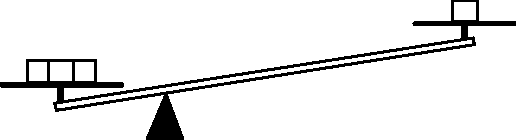
\includegraphics[width=0.35\textwidth]{Chapter4/简单的起重机械}
    \caption{简单的起重机械}
    \label{figure:简单的起重机械}
\end{wrapfigure}

我们设想存在着两类机械:一类是\uwave{不}可逆的,它包括所有的真实的机械;另一类是可逆的。当然实际上它是不可能达到的,不管我们怎样仔细地去设计轴承、杠杆等等。但是,我们假设有这样的东西——一台可逆机;在它使一个单位(一磅或任何其他单位)重的物体降低一个单位距离的时候提起了三个单位的重物。把这台可逆机称为A机。假定它使三个单位的重物升高的距离是$ x $。此外,假设还有另一台机械——B机,它不一定是可逆机,并且也使一个单位的重物降低一个单位距离,不过使三个单位的重物升高的距离是$ y $。我们现在可以证明$ y $不会高于$ x $,这就是说,不可能建造这样一种机械,能把重物抬得比可逆机所提到的高度还要\uwave{高}。让我们来看看为什么是这样。假设$ y $大于$ x $。我们用B机使一个单位的重物降低一个单位距离,这使三个单位的重物升高距离$y$,然后,我们可以使这个重物从$ y $降到$ x $获得\uwave{自由的能量},再利用可逆机A反向运转,使三个单位的重物降低$ x $而使一个单位的重物升高一个单位距离。这样一个单位的重物回到了原来的高度,而使这两台机械又处于初始的备用状态!因此,假如$ y $高于$ x $,那么就会有永恒运动,但我们已经假设这是不可能的。于是利用这些假定,我们就能够推导出\uwave{$ y $不会比$ x $}高,因此在所有可能设计的机械中,可逆机是最好的。

我们还可以看出所有的可逆机提升的高度一定\uwave{完全相同}。假定B的确也是可逆的。当然,前面关于$ y $不会高于$ x $的论据现在同样成立,但是我们也可以把这两台机械的工作顺序倒过来,即反之论证$ x $不高于$ y $。这一点是很值得注意的,因为它使我们能够在\uwave{不考察内部机制}的情况下分析不同的机械对物体可以提升的高度。我们立刻知道,如果有一个人制作了一组极其精巧的杠杆,利用这组杠杆使一个单位的重物降低一个单位距离就可以把三个单位的重物提升到某一个高度,把这组杠杆和一个具有同样用途的简单的可逆的杠杆作比较就可以知道它不会比简单的可逆的杠杆提得更高,而是或许还会低一些。假如这个人的机械是可逆的,我们也能精确地知道它可以提得\uwave{多}高。概括地说就是:每一台可逆机械无论怎样运转,当它使一个单位的重物下降一个单位距离时,总是会使三个单位的重物提升同样的距离$ x $。很清楚,这是一条非常有用的普遍定律。接下来的问题自然是$ x $是多少?

\begin{wrapfigure}{l}{0.45\textwidth}
    \centering
    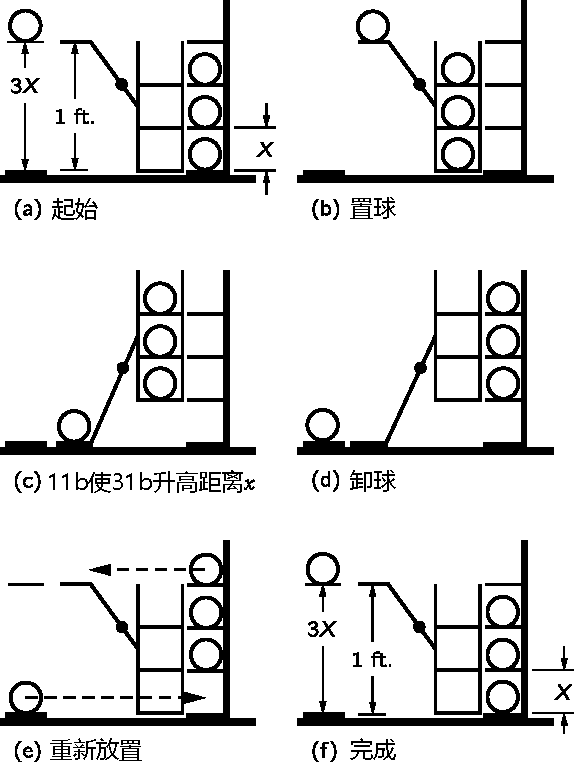
\includegraphics[width=0.42\textwidth]{Chapter4/一种可逆机}
    \caption{一种可逆机}
    \label{figure:一种可逆机}
\end{wrapfigure}

假如我们有一台可逆机,它能在3对1时提升距离$ x $。在图4.2中,我们在一个固定的多层架子上放置三个球。另外有一个球放在离地面一英尺的台上。这台机械可以使一个球降低1英尺来抬高三个球。现在,我们来这样安排:设容纳三个球的升降台有一层底板和两层架子,间隔正好是$ x $,其次,容纳球的多层架的间隔也是$ x $(图a)。首先我们使小球从多层架水平地滚到升降台上的架子中去(图b),我们假设这并不需要能量,因为高度并没有改变。于是开动可逆机进行工作:它使一个球降到底层,而使升降台升高距离$ x $(图c)。由于我们已经巧妙地安排了多层架,于是这些球又和架子相平。这样就把球卸到了多层架上(图 d)。卸了球以后,我们可以使机械回复到初始状态。现在在上面三层架子上有三个球,在底部有一个球,但是奇怪的是从某种观点上讲,我们根本没有使其中\uwave{两}个升高,因为,无论如何第二层和第三层架子像以前一样里面装着球。因此,最后的效果是使\uwave{一个}球升高了$ 3x$的距离。假如$  3x $超过1英尺,那么我们就可以把小球\uwave{放下来}使机械回到初始状态(图f),这样就能使这个装置再次运转。所以$ 3x $不可能超过1英尺,因为如果$ 3x $超过1英尺;我们就能创造出永恒运动。同样,使整台机械反向运行,我们可以证明,\uwave{1英尺不能超过$ 3x $},因为这是一台可逆机。所以\uwave{$ 3x $既不大于也不小于 1英尺},这样我们只是通过论证就发现了一条规律,$x=1/3$英尺。显然,这条规律可以推广为:开动一台可逆机使1磅重物降下一定距离,那么这台机械可以使$p$磅重物提高那段距离的$1/p$。另一种表示结果的说法是:3磅乘以所提高的距离(在我们的问题中是$ x $),等于1磅乘以所降低的距离(在这种情况下是1英尺)。如果我们先把所有的球的重量分别乘以它们现在所在的高度,然后使机械运转,再把所有的球的重量乘以它们所在的高度,得出的\uwave{前后结果不会有任何改变}。(我们必须把例子中只移动一个重物的情况推广到当我们降低一个重物就能提升几个不同的重物的情况——但这是不准的。)

我们把重量和高度的乘积之和称为\uwave{重力势能}——这是一个物体在空间上与地球之间的相互关系而具有的能量。那么,只要我们离地球不是太远(当位置很高时重力要减弱),重力势能的公式就是
\begin{equation}
    \label{Eq:I:4:3}
    \text{(一个物体的重力势能)}=
    \text{(重量)}\times\text{(高度)}
\end{equation}
这是一条十分优美的推理思路。唯一的问题在于,或许这并不是实际的情形。(无论如何,大自然\uwave{毋须}按我们的推理行事。)例如,也许永恒运动事实上是可能的。某些假设可能是错误的,或者我们的推理或许有错误,所以验证总是必要的。事实上,实验证明它是正确的。

那种与别的物体的相对位置有关的能量的一般名称就称为\uwave{势能}。当然,在上面的特殊情况中,我们则称它为\uwave{重力势能}。如果我们克服电力做功,而不是克服重力做功,即用许多杠杆“提升”一些电荷使之离开其他的电荷,那么所包含的能量就称为电势能。一般的原则是能量的变化为有关的力乘以力所推过的距离,而且这是一般的能量变化:
\begin{equation}
    \label{Eq:I:4:4}
    \text{(能量的变化)}=
    \text{(力)}\times\text{(力在作用下所通过的距离)}
\end{equation}
随着课程的进展我们还要讲到其余的种种势能。

\begin{figure}[htbp]
    \centering
    \begin{minipage}[t]{0.4\textwidth}
        \centering
        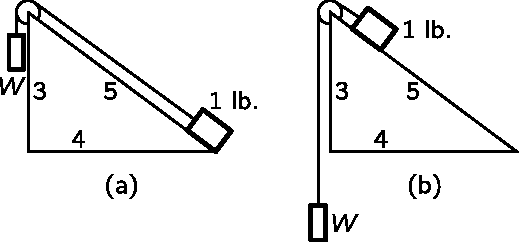
\includegraphics[width=6cm]{Chapter4/斜面}
        \caption{斜面}
    \end{minipage}
    \begin{minipage}[t]{0.4\textwidth}
        \centering
        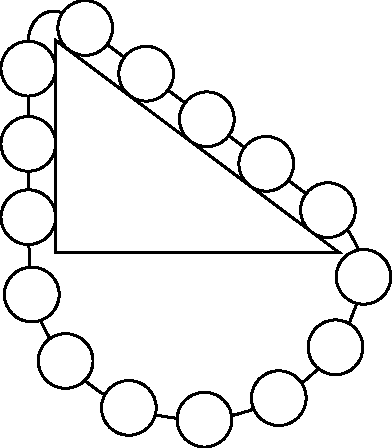
\includegraphics[width=6cm]{Chapter4/斯蒂维纽司的墓志铭}
        \caption{斯蒂维纽司的墓志铭}
    \end{minipage}
\end{figure}

在许多情况下能量守恒原理对于推断会发生什么事都是非常有用的。在高中你们已学过许多有关不同用途的滑轮和杠杆的定律,我们现在可以看到所有这些“定律”\uwave{都是一} \uwave{回事},并且不需要记住75条法则。一个简单的例子是如图4.3所示的一个光滑斜面,很巧,这是一个3--4--5的三角形。我们在斜面上用滑轮挂上一个1磅重的物体,而在滑轮的另一端悬挂一个重物$ W $。我们想知道为了平衡在斜面上的1磅重物,$ W $必须是多重?怎样来求出答案呢?假如我们说情况正好是平衡的话,那就是可逆的,因而可以使重物上下移动。所以,我们可以考虑下述情况。起初,如图(a)所示,1磅重物在斜面底部,而重物$ W $在斜面的顶端。当$ W $以一种可逆的方式滑下去后,1磅的物体就在斜面顶部,而$ W $经过的距离就是斜边的长度,如图(b)所示,即5英尺。我们使1磅重的重物只\uwave{提高}了3英尺而使W降低了\uwave{5英尺},所以,$ W=3/5 $磅。注意,我们是从\uwave{能量守恒},而不是从力的分解来得出这个斯蒂维纽司(Stevinus)所发现的方法就铭刻在他的墓碑上。图4.4说明这个重物一定是$ 3/5 $磅,因为这个圆球链并没有转动,很明显链条的下端的部分是为自身所平衡的,所以一边三个重物的拉力必须与另一边五个重物的拉力平衡,即按边长的比例。从图中你们可以看到,$W$一定是$ 3/5 $磅。

\begin{wrapfigure}{l}{0.4\textwidth}
    \centering
    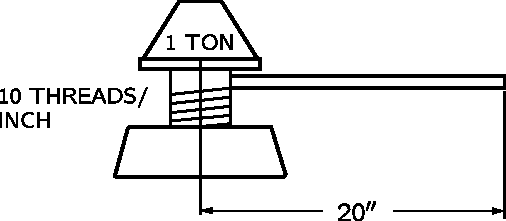
\includegraphics[width=0.35\textwidth]{Chapter4/螺旋起重器}
    \caption{螺旋起重器}
    \label{figure:螺旋起重器}
\end{wrapfigure}

让我们现在用图4.5所示的螺旋起重器这个比较复杂的问题来说明能量守恒原理。螺旋的把柄长为20英寸,螺纹为每英寸10圈,我们想知道,为了举起一吨(2000磅)的重物,在把柄上要施加多大的力?假如我们要使一吨重物升高1英寸,就必须使把柄转10圈。把柄转一次时大约走过126英寸。所以它总共要走过1260英寸,如果我们利用各种滑轮之类的机械,就可以用加在柄的端点上的一个未知的小重物$ W $来举起1吨的重物,我们发现,$ W $大约是1.6磅。这就是能量守恒的一个结果。

\begin{wrapfigure}{r}{0.4\textwidth}
    \centering
    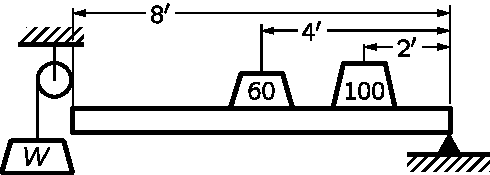
\includegraphics[width=0.35\textwidth]{Chapter4/一端支撑着的荷重杆}
    \caption{一端支撑着的荷重杆}
    \label{figure:一端支撑着的荷重杆}
\end{wrapfigure}

在图4.6中我们举一个稍为更复杂一点的例子。一根8英尺长的棒,一端被支撑着,在棒的中间有一个60磅的重物,离支点2英尺处有一个100磅的重物,假如不考虑棒的重量,为了保持它的平衡,我们要在棒的另一端加多大的力?假设在棒的那一端放上一个滑轮,并在滑轮上悬挂一个重物$ W $,为了使棒平衡,$ W $应当是多重?我们设想$ W $落下任意一段距离,为了简便起见,设它下降了4英寸,那么这两个重物要升高多少呢?棒的中心升高了2英寸,而离固定端2英寸处的那一点升高了1英寸,所以,各个重物与高度的乘积之和不变,这个原理告诉我们,$ W $乘以下降的4英寸,加上60磅乘以升高的2英寸,再加上100磅乘以升高的1英寸,其和必定是零。
\begin{equation}
    \label{Eq:I:4:5}
    -4W+(2)(60)+(1)(100)=0,\qquad
    W=\text{$55$ 磅}
\end{equation}
这就是说为了使棒平衡,必须加上一个55磅的重物。用这种方法,我们可以得出“平衡”定律——复杂的桥梁建筑的静力学,等等。这种处理问题的方法称为\uwave{虚功原理},因为为了进行这种论证,我们必须\uwave{设想}系统移动一下——即使它实际上没有移动,甚至不能移动。为了运用能量守恒的原理,我们用了很小的假想的运动。


\section{动能}

为了说明另一种形式的能量,我们来考虑一个单摆(图4.7)。假如我们把它拉向一边,再把它放开,它就会来回摆动。在这种运动中,每当从端点跑向中点时,它的高度降低了,这时势能跑到哪里去了呢?当摆降到底部时,势能就消失了,不过,它将再次爬上来。可见重力势能必定转变为另一种能量形式。很明显它是依靠了自己的\uwave{运动}才能重新爬上来。所以,当它到达底部时,重力势能就转变为某种其他形式的能量。

\begin{wrapfigure}{l}{0.4\textwidth}
    \centering
    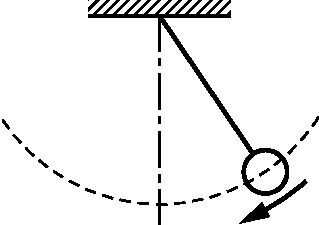
\includegraphics[width=0.35\textwidth]{Chapter4/单摆}
    \caption{单摆}
    \label{figure:单摆}
\end{wrapfigure}

我们应当得出一个运动能量的公式。现在,回想一下关于可逆机的论证,很容易看出,在底部的运动必定具有一定量的能量,可使摆升高到一定高度,这个能量与摆上升的\uwave{机制}无关,或者说与上升的路径无关,所以与我们对孩子玩积木的情形所写出的公式一样,这里也有一个(两种能量间的)等价公式。我们有另一种表示能量的形式,要说明它是不难的。摆在底部的动能等于重量乘以它能升高的高度:\text{K.E.}= WH。现在需要的是一个利用某种与物体的运动有关的规则来说明摆动高度的公式。假如我们以一定的速度直接朝上抛出一个物体,它将到达一定的高度;我们暂时还不知道到底是多高,但是它依赖于速度——关于这个,有一个相应的公式。于是,为了找到物体以速度$ V $运动的动能的公式,我们必须计算它能到达的高度;再乘以物体的重量。我们立刻就会知道,可以把动能写成这种形式:
\begin{equation}
    \label{Eq:I:4:6}
    K.E.=\frac{WV^2}{2g}
\end{equation}
当然,运动具有能量这个事实与物体处于重力场内这件事毫无关系。无论运动怎样产生,这都没有关系。这是一个适用于各种速度的一般公式。(\ref{Eq:I:4:3})及(\ref{Eq:I:4:6})两式都是近似的公式。(\ref{Eq:I:4:3})式在高度很大时是不正确的,因为这时,重力要减弱;而(\ref{Eq:I:4:6})在高速时要加以相对论性的校正。然而,当我们最后得到动能的精确公式时,能量守恒定律是正确的


\section{能量的其他形式}

我们可以继续以这种方法来说明能量还以其他的方式存在。首先考虑弹性能,假如我们拉伸弹簧,就必须作一些功,因为拉伸时,可以提起重物。所以弹簧在伸长的情况下具有做功的可能性。假如我们求出重量与高度的乘积之和,那将与总能量不符——我们必须加上另外的一些东西来说明弹簧处于拉紧状态这一事实。弹性能就是关于弹簧被伸长时这个事实的表述。它有多大呢?假如我们释放弹簧,那么弹簧经过平衡点时,弹性能就转变为动能,能量就在弹簧的伸长、压缩和动能之间来回变换。( 这里也有一些重力势能的增减,但是如果我们愿意的话,可以使实验“斜着”做)弹簧将一直来回振动,直到能量失掉为止……。啊哈!前面我们已经在整个过程中玩了一点小小的手法——如加上一些小重物使物体运动,或者说机械是可逆的,它们可以永远运动下去等。但是,我们可以看到这些东西最终都要停下来的。当弹簧不再上下振动时,能量到哪里去了呢?这就引进了另一种形式的能量:\uwave{热能}。

在弹簧或杠杆里有着由大量原子组成的晶体。假若极其仔细和精致地安排了机械的各个组成部分后,人们可以试着使事情作这样的调整:当某个东西在另一个东西上滚动时,根本没有一个原子会作任何跳动。但是我们必须非常小心。通常在机器运转时,由于材料本身的缺陷,会产生撞击和跳动,材料中的原子就开始无规则地摆动。于是那部分能量失踪了,但我们却发现机械运动减慢后,材料中的原子正以杂乱无章的方式摆动着,不错,这里仍然有动能,但是它与看得见的运动没有联系。多么奇怪!我们何以\uwave{知道}这里仍然有动能呢?我们发现,从温度计上可以看出,事实上弹簧或杠杆\uwave{变热}了,所以确实动能有了一定数量的增加。我们称这种形式的能量为\uwave{热能}。但是我们知道这实在并不是一种新的形式,它就是内部运动的动能。(我们在宏观范围内对物质所做的一切实验中都有一个困难,即不能真正演示出能量守恒,也不能实际制成可逆机,因为每当我们使大块材料运动时,原子不会绝对不受扰动,所以总有一定量的无规则运动进入原子系统,我们无法用眼睛看出这一点,但是可以用温度计或其他方式测量出来。)

还有许多其他形式的能量,当然,眼下不可能对它们叙述得更详细些。这里有电能,它与电荷的吸引和排斥有关。存在着一种辐射能,即光能,我们知道它是电能的一种,因为光可以表示为电磁场的振动;还有化学能——在化学反应中释放的能,它是原子彼此间相互吸引的能量。弹性能也是如此,所以实际上,弹性能在一定程度上就像化学能。我们目前对化学能的理解是化学能可分为两部分:首先是原子内电子的动能,所以化学能的一部分是动能,其余一部分是电子和质子的相互作用所产生的电能。接下去我们来考虑核能,它涉及原子核内的粒子的排列。我们有核能的公式,但是没有掌握基本的定律。我们知道它不是电能,不是重力能,也不纯粹是化学能,但是不知道它究竟是什么。看来这是另外的一种能量形式;最后,存在着一个与相对论有关的对动能定律的修正(或者你喜欢用的随便哪一种说法),也就是说动能与另一种称为\uwave{质能}的东西结合在一起。一个物体由于它的纯粹的\uwave{存在}就有能量产生。假如有一个静止的电子和一个静止的正电子起先稳定地搁置着而不发生任何作用——既不去考虑引力效应,也不去考虑其他,然后当它们碰在一起时就会湮没,并释放出一定量的辐射能,它是可以计算的。为此我们需要知道的只是物体的质量,而与究竟是什么物体无关。两个粒子消失后,就产生了一定的能量。爱因斯坦首先找到了计算公式,即$ E=mc^2 $。

从我们的讨论中可以很明显地看到,在进行分析时,能量守恒定律是极其有用的。我们已经在几个例子中表明了这一点,在那些例子中并没有知道所有的公式。假如我们有了各种能量的公式,那么毋须深入细节就能分析出有多少过程应当会发生。所以守恒定律是非常有趣的。由此很自然会产生一个问题,在物理学中还有哪些其他守恒定律?有另外两条守恒定律是与能量守恒定律类似的,一条称为线动量守恒,另一条称为角动量守恒,关于这方面我们在以后会知道得更多。归根到底,我们并没有深刻地理解守恒定律。我们不理解能量守恒,并不认为能量是一定数量的滴状物。你们也许听说过光子是以一个个的滴状形式出现的,一个光子的能量是普朗克常数乘以频率。这是正确的。但由于光的频率可以是任意的,所以没有哪条定律断言能量必须是某种确定的数值。与丹尼斯的积木不同,能量的数值可以是任意的,至少今天的理解是如此。所以在目前我们并不把能量理解为对某种东西的计数,而只是看作一种数学的量。这是一种抽象而又十分奇怪的情况。在量子力学中,我们知道能量守恒与世界的一个重要性质——事物不依赖于绝对时间——有十分密切的关系。我们可以在一个给定的时刻安排一个实验,并且完成它,然后在晚一些的时候再做同样的实验,那么实验的情形将完全是相同的。但这是否严格正确,我们并不知道。如果我们假设它\uwave{是}正确的,再加上量子力学的原理,我们就可以推导出能量守恒定律,这是一件相当微妙和有趣的事,不容易加以解释。其他的守恒定律也有联带的关系。动量守恒定律在量子力学中与一个命题有关,即无论你在\uwave{哪里}做实验都不会造成什么差别,结果总是同样的。最后,像空间上的无关性与动量守恒相联系、时间上的无关性与能量守恒相联系一样,假如我们\uwave{转动}仪器的话,这也不会造成任何差别,所以世界在角度取向上的不变性与\uwave{角动量守恒}相关。此外,还有三条其他的守恒定律。迄今为止我们可以说,这些定律是精确的。它们要容易理解得多,因为在本质上它们是属于清点积木一类的事。

这三条守恒定律中的第一条是电荷守恒定律这只是意味着,数一下你有多少正电荷,多少负电荷,将正电荷的数量减去负电荷的数量,那么这个结果将永远不会改变。你们可以用一个负电荷抵消一个正电荷,但是你们不可能创造任何正电荷对负电荷的净余额。另外两条守恒定律与这一条相类似。一条称为\uwave{重子的守恒}。存在着一些奇异粒子,例如中子和质子,它们称为重子。在任何自然界的反应中,假如我们数一下有多少重子进入一个反应,那么在反应结束时出去的重子\footnote{反重子的重子数记为(-1)}的数量将完全相同。还有一条是轻子守恒定律。我们可以举出称为轻子的一群粒子:电子,μ介子和中微子,还有一个电子的反粒子,即正电子(轻子数为-1)。在一个反应中对轻子的总数进行计数将揭示出这个事实:进入的数量与出去的数量决不会改变,至少就今天所知就是如此。

这就是六条守恒定律,其中三条是微妙的,与空间和时间有关,另外三条从对某种东西进行计数的意义上说是简单的。

关于能量守恒,我们应当指出,可资利用的能量是另一回事——在海水中的原子进行着大量的晃动,因为海水具有一定的温度,但是如果不从别处取得能量,就不可能使原子都按一个确定的方向运动。这就是说:虽然我们知道能量确实守恒,但是可供人类利用的能量并不那么易于保存。确定究竟有多少能量可供利用的那些定律称为\uwave{热力学定律},它们包括着一个称为熵的有关不可逆热力学过程的概念。

最后,我们提一下这个问题:今天我们可以从哪里获得能量的供应?我们的能量来源是太阳、雨水、煤、铀以及氢。大阳形成了降雨,也造成了煤矿,所以所有这些都起源于太阳。虽然能量是守恒的,但看来大自然对此并无兴趣,她使太阳释放了大量的能量,但其中只有二十亿分之一到达地球。大自然保存着能量,不过实际上并不关心这一点;她让巨大数量的能量向四面八方散布开去。我们已经从铀中得到能量,从氢中也能得到能量,但是,现在只是在爆炸的危险的条件下才得到这些能量。假如可以在热核反应中控制它,那么结果每秒钟从10夸脱水中得到的能量就等于整个美国每秒钟所发的电量,每分钟用150加仑的水,就会使你们有足够的燃料来供应今天在整个美国所需要使用的能量!所以,怎样想出一些办法使我们从对能量的需要中解放出来就成为物理学家的责任。无疑,这是可以达到的目标。
